% This example is meant to be compiled with lualatex or xelatex
% The theme itself also supports pdflatex
\PassOptionsToPackage{unicode}{hyperref}
\documentclass[aspectratio=1610, xcolor=dvipsnames, 9pt]{beamer}

% Load packages you need here
\usepackage{polyglossia}
\setmainlanguage{german}

\usepackage{csquotes}
\usepackage{smartdiagram}

\usepackage{amsmath}
\usepackage{amssymb}
\usepackage{mathtools}

\usepackage{hyperref}
\usepackage{bookmark}

% load the theme after all packages

\usetheme[
  showtotalframes, % show total number of frames in the footline
]{fhswf}

% Put settings here, like
\unimathsetup{
  math-style=ISO,
  bold-style=ISO,
  nabla=upright,
  partial=upright,
  mathrm=sym,
}

\title{Advanced Natural Language Processing/ Large Language Models}
\author[F.~Neubürger]{ \textbf{Felix Neubürger}}
\institute[I \& W]{Fachhochschule Südwestfalen, Ingenieurs- \& Wirtschaftswissenschaften}
\date{2025}
\titlegraphic{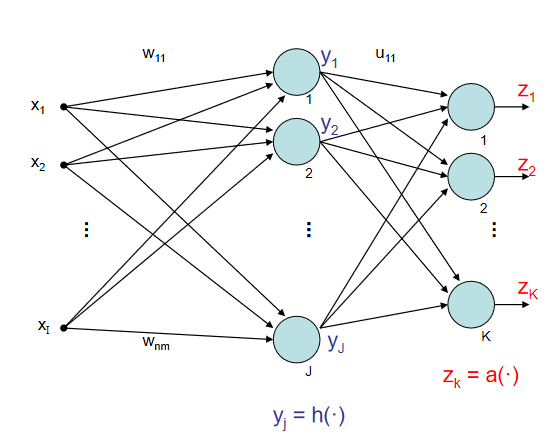
\includegraphics[width=0.2\textwidth]{images/MLP2.png}}


\begin{document}

\maketitle
\begin{frame}{Abfrage Erwartungen und Vorwissen}
  \begin{columns}
    \begin{column}{1\textwidth}
      \begin{itemize}
        \item \url{https://www.menti.com/} \newline
        \item Code: 3972 7236
      \end{itemize}
    \end{column}
    \begin{column}{0\textwidth}
% \begin{figure}
% \centering
%             \includegraphics[width=0.9\textwidth]{images/intro/intro.pdf}
% \end{figure}
    \end{column}
  \end{columns}
\end{frame}

\begin{frame}{Inhalte der Vorlesung}
  \begin{columns}
    \begin{column}{1\textwidth}
      \begin{itemize}
        \item Wie funktioniert Natural Language Processing\newline
        \item Sprachdarstellung zum Rechnen \newline
        \item Attentionmechanismus \newline
        \item Transformerarchitektur  \newline
        \item von BERT zu DeepSeek-v3 \newline 
        \item Wie es weitergehen kann \newline
        \item Nutzungsmöglichkeiten: RAG, Agentensysteme \newline
        \item Strategien zur Durchführung von PM Projekten
      \end{itemize}
    \end{column}
    \begin{column}{0\textwidth}
% \begin{figure}
% \centering
%             \includegraphics[width=0.9\textwidth]{images/intro/intro.pdf}
% \end{figure}
    \end{column}
  \end{columns}
\end{frame}

\begin{frame}{Ziele der Vorlesung - Welche Fragen sollen beantwortet werden?}
  \begin{columns}
    \begin{column}{0.69\textwidth}
      \begin{itemize}
        \item Was genau machen Neuronale Netze? \newline
        \item Wie kann ich mir das vorstellen? \newline
        \item Was ist überhaupt "Deep Learning"?  \newline
        %\item Welche Vorteile kann Predictive Maintenance haben? \newline
        \item Welche verschiedenen Architekturen neuronaler Netze gibt es? \newline
        \item Muss es immer Deep Learning sein? \newline
        %\item Wie gehe ich an ein Predictive Maintenance Projekt heran?
      \end{itemize}
    \end{column}
    \begin{column}{0.3\textwidth}
 \begin{figure}
 \centering
             
\includegraphics[width=0.9\textwidth]{images/ai_methodology.png}
             [\url{https://xkcd.com/2451/}]
 \end{figure}
    \end{column}
  \end{columns}
\end{frame}

\begin{frame}{Format der Vorlesung - Wie sollen diese Fragen beantwortet werden?}
  \begin{columns}
    \begin{column}{0.69\textwidth}
      \begin{itemize}
        \item Theroretischer Teil mit Folien \newline
        \item Praktischer Teil in Gruppen an einem Projekt  \newline
        \item Gruppengröße 2 oder 3 Personen  \newline
        %\item Welche Vorteile kann Predictive Maintenance haben? \newline
        \item Einzelarbeit möglich wenn eigenes Thema vorhanden \newline
        \item Abgabe der Ausarbeitung einen Tag vor der Veranstaltung in der Blockwoche \newline
        \item Vorstellung der Projektergebnisse in der Blockwoche \newline
        \item Gewichtung der Bewertung Projektausarbeitung (70\%) und Vortrag (30\%)
        %\item Wie gehe ich an ein Predictive Maintenance Projekt heran?
      \end{itemize}
    \end{column}
    \begin{column}{0.3\textwidth}
 \begin{figure}
 \centering
             
\includegraphics[width=0.7\textwidth]{images/tasks.png} \newline
             [\url{https://xkcd.com/1425/}]
 \end{figure}
    \end{column}
  \end{columns}
\end{frame}

\begin{frame}{LLM Standardwerke}
\begin{itemize}
\item \textbf{Build LLMs from Scratch} (Raschka)
\begin{itemize}
\item \url{https://github.com/rasbt/LLMs-from-scratch}
\item Praktische Implementierung in PyTorch
\end{itemize}

\item \textbf{Transformers for NLP} (Rothman)
\begin{itemize}
\item ISBN 978-1803247335
\item BERT/GPT Anwendungen
\end{itemize}
\end{itemize}
\end{frame}

\begin{frame}{LLM Forschungsarbeiten}
\begin{itemize}
\item \textbf{Attention Is All You Need} (2017)
\begin{itemize}
\item \url{https://arxiv.org/abs/1706.03762}
\item Transformer-Architektur
\end{itemize}

\item \textbf{BERT Paper} (Devlin 2019)
\begin{itemize}
\item \url{https://arxiv.org/abs/1810.04805}
\item Bidirektionale Pretraining
\end{itemize}

\item \textbf{GPT-3 Paper} (Brown 2020)
\begin{itemize}
\item \url{https://arxiv.org/abs/2005.14165}
\item Few-Shot Learning
\end{itemize}
\end{itemize}
\end{frame}

\begin{frame}{LLM Praktische Ressourcen}
\begin{itemize}
\item \textbf{Hugging Face Transformers}
\begin{itemize}
\item \url{https://github.com/huggingface/transformers}
\end{itemize}

\item \textbf{LangChain}
\begin{itemize}
\item \url{https://python.langchain.com/}
\item LLM Orchestrierung
\end{itemize}

\item \textbf{LLaMA \& LlamaIndex}
\begin{itemize}
\item \url{https://github.com/facebookresearch/llama}
\item Open-Weight Modelle
\end{itemize}
\end{itemize}
\end{frame}
\begin{frame}[allowframebreaks]{References}
 \bibliographystyle{ieeetr}
 \bibliography{lit.bib}
\end{frame}
\end{document}
